\section{Entity--Relationship Diagram}
In order to have an idea of how the database handles bookings, location of bicycles, and their relation to the location of the stations, an ER Diagram was made, see \figref{fig:er-dia}.

\begin{figure}
	\centering
	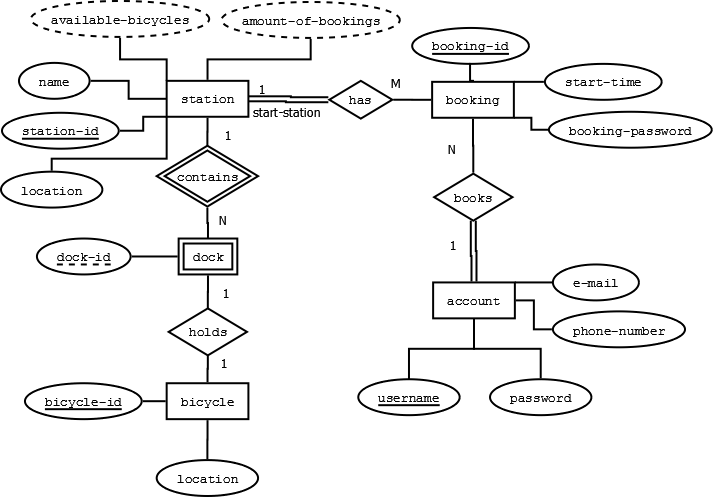
\includegraphics[scale=0.4]{relevantmaterial/erdiagram}
	\caption{The ER Diagram for database overview. Does not include less important attributes.}\label{fig:er-dia}
\end{figure}

As seen in the diagram, the entities consists of bicycle, dock, station, booking, and account.
An account consists of a username, email, which both must be unique, a phone-number, and password.
These attributes are common for an account entity, with the phone-number being special in that the idea is they will receive the booking-password over SMS.

In relation to this is the booking entity, where it can be seen that a user can have many bookings whereas a booking is registered to one and only one account.
The booking then has a booking-id, to uniquely identify a booking, a start-time, such that a station knows when to lock a bicycle, and a booking-password, used to unlock a bicycle at the given start-time if a correct password is entered.
The idea is that if a booking is not used in a given time frame at the start-time, the booking will be removed, to prevent spamming of bookings without use.

A booking is also tied to a station, such that a booking is located at one and only one station, whereas a station can have many bookings.

A station has the attribute station-id, to uniquely identify the station.
Furthermore, it has a name, which is thought to be used to give a meaningful description of a given station.
We are aware that the name could be used as a primary key, but having an id as the primary key unlocks the possibility of duplicate names, which might be desired for stations located at different spots in the city, example could be two stations named "AAU Bycykel Station" which is a quite generic name.

In addition to this, a station has a location, which is used to easily place a station on a map, and can also be used for calculations such as distance between a given station and bicycle.
A station also has two derived attributes, which are available-bicycles and amount-of-bookings, these are attributes that is beneficial to show to the user, such that they can see if it is possible to gather a bicycle at a given station.

Next is the dock entity, which is a weak entity, as it cannot exist without a station.
This represents the real-life situation with stations located around the city, and each of these has a number of docks.
The dock only has one attribute, which is the dock-id, used to identify a dock in combination with a station-id.

The interesting part of a dock is its relation with a bicycle.
A dock may or may not hold a bicycle, which is represented with the holds relation.\fxwarning{Locked docks?}

The bicycle entity then consists of a bicycle-id, to uniquely identify a given bicycle, and a location, which can be used to locate lost bicycles.